\documentclass[11pt]{article}
\usepackage[notes]{la}
\lamodule{5}{1}{Eigenvectors and Eigenvalues}
\laxdoc{1.4}
\laxdoc{1.7}
\laxdoc{2.3}
\laxdoc{2.2}
\laxdoc{4.2}
\laxdoc{4.3}
\laxdoc{4.5}

\begin{document}

\section{Eigenvectors and Eigenvalues}

\begin{guide}
Multiply a vector by a matrix and, in general, the vector is both turned and stretched: $A\bv{x}$ points in a new direction. Is there ever a vector that is \emph{only} stretched, so that $A\bv{x}$ lies on the same line through the origin as $\bv{x}$? If such vectors exist, a matrix can be understood one line at a time, and the line is described by a single number, the stretch factor. This section finds those lines, shows that they come with a subspace attached, and shows how many of them a matrix can have. Throughout, $A$ is a square matrix, because $A\bv{x}$ and $\bv{x}$ must live in the same space to be compared.
\end{guide}

\textbf{By the end of this section you should be able to:}
\begin{itemize}
  \item state the definition of an eigenvector and an eigenvalue, and decide whether a given vector is an eigenvector of a given matrix by computing $A\bv{x}$ and comparing it with $\bv{x}$;
  \item decide whether a given scalar is an eigenvalue by row reducing $[\,A-\lambda I\ \ \bv{0}\,]$, and explain why this works;
  \item find a basis for the eigenspace of a known eigenvalue, and say how the dimension of an eigenspace is read from the free variables;
  \item explain why $0$ is an eigenvalue exactly when $A$ is not invertible, and why the eigenvalues of a triangular matrix are its diagonal entries;
  \item prove and use the theorem that eigenvectors for different eigenvalues are linearly independent, and conclude that an $n\times n$ matrix has at most $n$ different eigenvalues;
  \item recognise eigenvectors and eigenvalues of a linear transformation of a vector space such as $\mathbb{P}_n$, $M_{2\times2}$ or a space of functions.
\end{itemize}

% ---------------------------------------------------------------------
\subsection*{Vectors that keep their direction}

Start with one matrix and look at what it does to three vectors of $\R^2$.

\begin{exmp}{A matrix that stretches some lines and turns others}{first}
Let $A=\begin{bmatrix}4&1\\2&3\end{bmatrix}$ and take $\bv{u}=(1,0)$, $\bv{v}=(1,1)$, $\bv{w}=(1,-2)$. Then
\[
A\bv{u}=\begin{bmatrix}4\\2\end{bmatrix},\qquad
A\bv{v}=\begin{bmatrix}4+1\\2+3\end{bmatrix}=\begin{bmatrix}5\\5\end{bmatrix}=5\begin{bmatrix}1\\1\end{bmatrix},\qquad
A\bv{w}=\begin{bmatrix}4-2\\2-6\end{bmatrix}=\begin{bmatrix}2\\-4\end{bmatrix}=2\begin{bmatrix}1\\-2\end{bmatrix}.
\]
The vector $\bv{u}$ is turned: $(4,2)$ is not a multiple of $(1,0)$. The vector $\bv{v}$ is only stretched, by the factor $5$, and $\bv{w}$ is only stretched, by the factor $2$. So $A$ acts on the line through $\bv{v}$ as ``multiply by $5$'' and on the line through $\bv{w}$ as ``multiply by $2$''. Every vector on those two lines behaves the same way, because $A(c\bv{v})=cA\bv{v}=5(c\bv{v})$.
\end{exmp}

\begin{center}
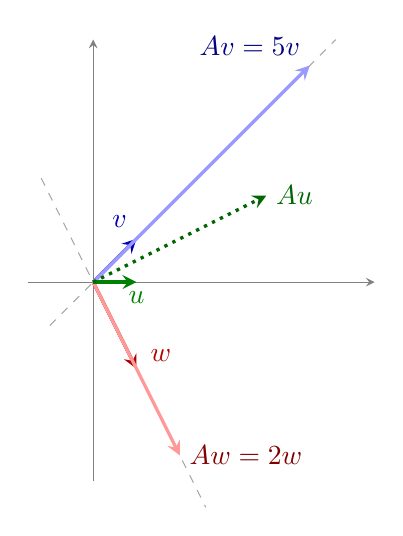
\begin{tikzpicture}[x=0.55cm,y=0.55cm,>=stealth]
  \draw[->,gray] (-1.5,0)--(6.5,0);
  \draw[->,gray] (0,-4.6)--(0,5.6);
  \draw[dashed,gray!70] (-1,-1)--(5.6,5.6);
  \draw[dashed,gray!70] (-1.2,2.4)--(2.6,-5.2);
  \draw[->,very thick,blue!70!black] (0,0)--(1,1);
  \draw[->,very thick,blue!40] (0,0)--(5,5);
  \draw[->,very thick,red!70!black] (0,0)--(1,-2);
  \draw[->,very thick,red!40] (0,0)--(2,-4);
  \draw[->,very thick,green!50!black] (0,0)--(1,0);
  \draw[->,very thick,green!40!black,dotted] (0,0)--(4,2);
  \node[blue!70!black,left] at (1,1.4) {$v$};
  \node[blue!50!black,above left] at (5,5) {$Av=5v$};
  \node[red!70!black,right] at (1.1,-1.7) {$w$};
  \node[red!50!black,right] at (2,-4) {$Aw=2w$};
  \node[green!50!black,below] at (1,0) {$u$};
  \node[green!40!black,right] at (4,2) {$Au$};
\end{tikzpicture}
\end{center}

\noindent\textbf{Figure 1.} The vectors $\bv{v}$ and $\bv{w}$ of Example~\ref{ex:first} stay on their lines (dashed) when $A$ acts; $\bv{u}$ leaves its line.

\begin{defn}{Eigenvector and eigenvalue}{eigen}
Let $A$ be an $n\times n$ matrix. An \emph{eigenvector} of $A$ is a \emph{nonzero} vector $\bv{x}$ in $\R^n$ such that
\[
A\bv{x}=\lambda\bv{x}\qquad\text{for some scalar }\lambda.
\]
The scalar $\lambda$ is then called an \emph{eigenvalue} of $A$, and $\bv{x}$ is an eigenvector \emph{for} (or \emph{belonging to}) $\lambda$. A scalar $\lambda$ is an eigenvalue of $A$ if and only if the equation $A\bv{x}=\lambda\bv{x}$ has a solution $\bv{x}\neq\bv{0}$.
\end{defn}

In Example~\ref{ex:first}, $5$ is an eigenvalue of $A$ with the eigenvector $(1,1)$, and $2$ is an eigenvalue with the eigenvector $(1,-2)$. The prefix ``eigen'' is German for ``own'' or ``characteristic'': the eigenvectors are the vectors that the matrix treats most simply.

\begin{think}{Why nonzero?}{nonzero}
(a)~Show that $A\bv{0}=\lambda\bv{0}$ holds for \emph{every} scalar $\lambda$ and every matrix $A$. What would go wrong with the definition if $\bv{0}$ were allowed as an eigenvector? (b)~Is the scalar $\lambda=0$ allowed to be an eigenvalue? What does $A\bv{x}=0\bv{x}$ say about $\bv{x}$?
\end{think}

\begin{exmp}{Is a given vector an eigenvector?}{test}
Let $B=\begin{bmatrix}2&-1&1\\4&3&1\\4&2&2\end{bmatrix}$, $\bv{p}=(-2,2,4)$ and $\bv{q}=(1,1,1)$. To test a vector, multiply and compare:
\[
B\bv{p}=\begin{bmatrix}2&-1&1\\4&3&1\\4&2&2\end{bmatrix}\begin{bmatrix}-2\\2\\4\end{bmatrix}=\begin{bmatrix}-4-2+4\\-8+6+4\\-8+4+8\end{bmatrix}=\begin{bmatrix}-2\\2\\4\end{bmatrix}=1\cdot\bv{p},
\]
so $\bv{p}$ is an eigenvector of $B$ for the eigenvalue $1$. But
\[
B\bv{q}=\begin{bmatrix}2&-1&1\\4&3&1\\4&2&2\end{bmatrix}\begin{bmatrix}1\\1\\1\end{bmatrix}=\begin{bmatrix}2\\8\\8\end{bmatrix},
\]
and $(2,8,8)$ is not a multiple of $(1,1,1)$ (a multiple $\lambda(1,1,1)$ has three equal entries), so $\bv{q}$ is not an eigenvector. The test is: compute $A\bv{x}$, then ask whether it is a scalar multiple of $\bv{x}$.
\end{exmp}

\begin{kc}{Test the vectors}{vec}
Let $A=\begin{bmatrix}3&-2\\1&0\end{bmatrix}$. For each vector decide whether it is an eigenvector of $A$, and if so give the eigenvalue: (a)~$(1,1)$; (b)~$(2,1)$; (c)~$(1,2)$; (d)~$(-4,-2)$.
\end{kc}

\subsection*{Is this number an eigenvalue? Eigenspaces}

The definition tests a \emph{vector}. To test a \emph{scalar}, we turn $A\bv{x}=\lambda\bv{x}$ into a homogeneous system. Since $\lambda\bv{x}=\lambda I\bv{x}$,
\[
A\bv{x}=\lambda\bv{x}\iff A\bv{x}-\lambda I\bv{x}=\bv{0}\iff (A-\lambda I)\bv{x}=\bv{0}.
\]

\begin{thm}{Testing a scalar}{test}
Let $A$ be an $n\times n$ matrix and $\lambda$ a scalar. The following statements are equivalent.
\begin{enumerate}[label=(\alph*),itemsep=1pt]
  \item $\lambda$ is an eigenvalue of $A$.
  \item The equation $(A-\lambda I)\bv{x}=\bv{0}$ has a nontrivial solution.
  \item $A-\lambda I$ is not invertible.
  \item The columns of $A-\lambda I$ are linearly dependent.
\end{enumerate}
Moreover, the eigenvectors of $A$ for $\lambda$ are exactly the nonzero solutions of $(A-\lambda I)\bv{x}=\bv{0}$. In particular, $0$ is an eigenvalue of $A$ if and only if $A$ is not invertible.
\end{thm}

\begin{proof}
By the computation above, $A\bv{x}=\lambda\bv{x}$ and $(A-\lambda I)\bv{x}=\bv{0}$ are the same equation, so the same vectors solve them. An eigenvector for $\lambda$ is a \emph{nonzero} solution, which gives the last sentence and the equivalence of (a) and (b). Statements (b) and (c) are equivalent by the Invertible Matrix Theorem (Theorem~\ref{2.3-thm:imt}): a square matrix is invertible exactly when its homogeneous equation has only the trivial solution. Statements (b) and (d) are equivalent by Theorem~\ref{1.7-thm:cols}. Finally, take $\lambda=0$: then $A-0I=A$, and (c) says that $A$ is not invertible.
\end{proof}

\begin{exmp}{Is $4$ an eigenvalue of $B$? Is $3$?}{isvalue}
Use $B$ from Example~\ref{ex:test}. By Theorem~\ref{thm:test}, $4$ is an eigenvalue exactly when $(B-4I)\bv{x}=\bv{0}$ has a nontrivial solution. Row reduce $[\,B-4I\ \ \bv{0}\,]$:
\begin{align*}
\begin{amat}{ccc|c}-2 & -1 & 1 & 0\\4 & -1 & 1 & 0\\4 & 2 & -2 & 0\end{amat}
&\rops{-\tfrac{1}{2}R_1}
\begin{amat}{ccc|c}1 & \tfrac{1}{2} & -\tfrac{1}{2} & 0\\4 & -1 & 1 & 0\\4 & 2 & -2 & 0\end{amat}
\rops{R_2-4R_1,\ R_3-4R_1}
\begin{amat}{ccc|c}1 & \tfrac{1}{2} & -\tfrac{1}{2} & 0\\0 & -3 & 3 & 0\\0 & 0 & 0 & 0\end{amat}
\\[4pt]
&\rops{-\tfrac{1}{3}R_2}
\begin{amat}{ccc|c}1 & \tfrac{1}{2} & -\tfrac{1}{2} & 0\\0 & 1 & -1 & 0\\0 & 0 & 0 & 0\end{amat}
\rops{R_1-\tfrac{1}{2}R_2}
\begin{amat}{ccc|c}1 & 0 & 0 & 0\\0 & 1 & -1 & 0\\0 & 0 & 0 & 0\end{amat}
\end{align*}
The third column has no pivot, so $x_3$ is free and there are nontrivial solutions: $x_1=0$ and $x_2=x_3$. With $x_3=1$ we get the eigenvector $(0,1,1)$. Check: $B(0,1,1)=(-1+1,\ 3+1,\ 2+2)=(0,4,4)=4(0,1,1)$. \ $\checkmark$ So $4$ is an eigenvalue.

Now test $3$. Row reduce $[\,B-3I\ \ \bv{0}\,]$:
\begin{align*}
\begin{amat}{ccc|c}-1 & -1 & 1 & 0\\4 & 0 & 1 & 0\\4 & 2 & -1 & 0\end{amat}
&\rops{-R_1}
\begin{amat}{ccc|c}1 & 1 & -1 & 0\\4 & 0 & 1 & 0\\4 & 2 & -1 & 0\end{amat}
\rops{R_2-4R_1,\ R_3-4R_1}
\begin{amat}{ccc|c}1 & 1 & -1 & 0\\0 & -4 & 5 & 0\\0 & -2 & 3 & 0\end{amat}
\\[4pt]
&\rops{-\tfrac{1}{4}R_2}
\begin{amat}{ccc|c}1 & 1 & -1 & 0\\0 & 1 & -\tfrac{5}{4} & 0\\0 & -2 & 3 & 0\end{amat}
\rops{R_1-R_2,\ R_3+2R_2}
\begin{amat}{ccc|c}1 & 0 & \tfrac{1}{4} & 0\\0 & 1 & -\tfrac{5}{4} & 0\\0 & 0 & \tfrac{1}{2} & 0\end{amat}
\\[4pt]
&\rops{2R_3}
\begin{amat}{ccc|c}1 & 0 & \tfrac{1}{4} & 0\\0 & 1 & -\tfrac{5}{4} & 0\\0 & 0 & 1 & 0\end{amat}
\rops{R_1-\tfrac{1}{4}R_3,\ R_2+\tfrac{5}{4}R_3}
\begin{amat}{ccc|c}1 & 0 & 0 & 0\\0 & 1 & 0 & 0\\0 & 0 & 1 & 0\end{amat}
\end{align*}
Every column has a pivot, so only $\bv{x}=\bv{0}$ solves $(B-3I)\bv{x}=\bv{0}$, and $3$ is \emph{not} an eigenvalue of $B$. (The pivot positions decide: a free variable means an eigenvalue, no free variable means none.)
\end{exmp}

\begin{kc}{Is the scalar an eigenvalue?}{scalar}
Let $A=\begin{bmatrix}1&2\\3&2\end{bmatrix}$. (a)~Is $4$ an eigenvalue? If so, find an eigenvector. (b)~Is $2$ an eigenvalue? (c)~Is $0$ an eigenvalue? Which theorem lets you answer (c) without row reducing?
\end{kc}

\begin{defn}{Eigenspace}{eigspace}
Let $\lambda$ be an eigenvalue of the $n\times n$ matrix $A$. The \emph{eigenspace} of $A$ for $\lambda$ is the null space of $A-\lambda I$:
\[
E_\lambda=\Nul(A-\lambda I)=\{\bv{x}\in\R^n:\ A\bv{x}=\lambda\bv{x}\}.
\]
It consists of all eigenvectors for $\lambda$, together with the zero vector.
\end{defn}

\begin{thm}{An eigenspace is a subspace}{eigsub}
The eigenspace $E_\lambda$ is a subspace of $\R^n$. Hence any linear combination of eigenvectors for the same eigenvalue $\lambda$ is again an eigenvector for $\lambda$, or is $\bv{0}$.
\end{thm}

\begin{proof}
$E_\lambda=\Nul(A-\lambda I)$ is the null space of an $n\times n$ matrix, and a null space is a subspace (Theorem~\ref{4.2-thm:nulsub}). The second sentence is closure of a subspace under linear combinations: a combination of vectors with $A\bv{x}=\lambda\bv{x}$ also satisfies this equation, and if it is not $\bv{0}$ it is an eigenvector by Definition~\ref{def:eigen}.
\end{proof}

The theorem has a warning built in. Two eigenvectors for \emph{different} eigenvalues need not combine into an eigenvector (Pause and think~\ref{think:sum}); only vectors for the \emph{same} eigenvalue can be mixed.

\begin{think}{Mixing eigenvectors}{sum}
(a)~For $A=\begin{bmatrix}4&1\\2&3\end{bmatrix}$ of Example~\ref{ex:first}, let $\bv{v}=(1,1)$ (eigenvalue $5$) and $\bv{w}=(1,-2)$ (eigenvalue $2$). Compute $A(\bv{v}+\bv{w})$ and decide whether $\bv{v}+\bv{w}$ is an eigenvector. (b)~Which step of the proof of Theorem~\ref{thm:eigsub} fails when the two eigenvalues are different?
\end{think}

\begin{proc}{Finding a basis for the eigenspace of a known eigenvalue}{eigspace}
\begin{enumerate}[itemsep=1pt]
  \item Form the matrix $A-\lambda I$ (subtract $\lambda$ from each diagonal entry).
  \item Row reduce $[\,A-\lambda I\ \ \bv{0}\,]$ to reduced echelon form.
  \item If there is no free variable, $\lambda$ is not an eigenvalue. Otherwise write the solutions in parametric vector form; the vectors multiplying the free variables form a basis for $E_\lambda$ (Theorem~\ref{4.3-thm:nulbasis}), and $\dim E_\lambda$ is the number of free variables.
\end{enumerate}
\end{proc}

\begin{exmp}{Both eigenspaces of the first matrix}{eigspaces2}
For $A=\begin{bmatrix}4&1\\2&3\end{bmatrix}$ we found the eigenvalues $5$ and $2$ by luck. Now the eigenspaces. For $\lambda=5$:
\begin{align*}
\begin{amat}{cc|c}-1 & 1 & 0\\2 & -2 & 0\end{amat}
&\rops{-R_1}
\begin{amat}{cc|c}1 & -1 & 0\\2 & -2 & 0\end{amat}
\rops{R_2-2R_1}
\begin{amat}{cc|c}1 & -1 & 0\\0 & 0 & 0\end{amat}
\end{align*}
Here $x_2$ is free and $x_1=x_2$, so $E_5=\Span\{(1,1)\}$. For $\lambda=2$:
\begin{align*}
\begin{amat}{cc|c}2 & 1 & 0\\2 & 1 & 0\end{amat}
&\rops{\tfrac{1}{2}R_1}
\begin{amat}{cc|c}1 & \tfrac{1}{2} & 0\\2 & 1 & 0\end{amat}
\rops{R_2-2R_1}
\begin{amat}{cc|c}1 & \tfrac{1}{2} & 0\\0 & 0 & 0\end{amat}
\end{align*}
Here $x_2$ is free and $x_1=-\tfrac12x_2$; taking $x_2=-2$ to clear the fraction gives $E_2=\Span\{(1,-2)\}$. Each eigenspace is a line through the origin, which is exactly what Figure~1 showed.
\end{exmp}

\begin{exmp}{An eigenspace of dimension two}{eig2dim}
Let $A=\begin{bmatrix}-1&4&0\\0&3&0\\-4&4&3\end{bmatrix}$. Then $3$ is an eigenvalue; to find $E_3$, row reduce $[\,A-3I\ \ \bv{0}\,]$:
\begin{align*}
\begin{amat}{ccc|c}-4 & 4 & 0 & 0\\0 & 0 & 0 & 0\\-4 & 4 & 0 & 0\end{amat}
&\rops{-\tfrac{1}{4}R_1}
\begin{amat}{ccc|c}1 & -1 & 0 & 0\\0 & 0 & 0 & 0\\-4 & 4 & 0 & 0\end{amat}
\rops{R_3+4R_1}
\begin{amat}{ccc|c}1 & -1 & 0 & 0\\0 & 0 & 0 & 0\\0 & 0 & 0 & 0\end{amat}
\end{align*}
The variables $x_2$ and $x_3$ are free and $x_1=x_2$, so
\[
\bv{x}=\begin{bmatrix}x_2\\x_2\\x_3\end{bmatrix}=x_2\begin{bmatrix}1\\1\\0\end{bmatrix}+x_3\begin{bmatrix}0\\0\\1\end{bmatrix},
\]
and $\{(1,1,0),(0,0,1)\}$ is a basis for $E_3$, which is a plane through the origin: $\dim E_3=2$. Check both vectors: $A(1,1,0)=(-1+4,\ 3,\ -4+4)=(3,3,0)=3(1,1,0)$ and $A(0,0,1)=(0,0,3)=3(0,0,1)$. \ $\checkmark$ For $\lambda=-1$:
\begin{align*}
\begin{amat}{ccc|c}0 & 4 & 0 & 0\\0 & 4 & 0 & 0\\-4 & 4 & 4 & 0\end{amat}
&\rops{R_1\leftrightarrow R_3}
\begin{amat}{ccc|c}-4 & 4 & 4 & 0\\0 & 4 & 0 & 0\\0 & 4 & 0 & 0\end{amat}
\rops{-\tfrac{1}{4}R_1}
\begin{amat}{ccc|c}1 & -1 & -1 & 0\\0 & 4 & 0 & 0\\0 & 4 & 0 & 0\end{amat}
\\[4pt]
&\rops{\tfrac{1}{4}R_2}
\begin{amat}{ccc|c}1 & -1 & -1 & 0\\0 & 1 & 0 & 0\\0 & 4 & 0 & 0\end{amat}
\rops{R_1+R_2,\ R_3-4R_2}
\begin{amat}{ccc|c}1 & 0 & -1 & 0\\0 & 1 & 0 & 0\\0 & 0 & 0 & 0\end{amat}
\end{align*}
Here $x_3$ is free, $x_1=x_3$ and $x_2=0$, so $E_{-1}=\Span\{(1,0,1)\}$ (check: $A(1,0,1)=(-1,0,-4+3)=(-1,0,-1)=-(1,0,1)$ \ $\checkmark$).
\end{exmp}

\begin{think}{Dimension and free variables}{freevars}
(a)~In Example~\ref{ex:eig2dim} the matrix $A-3I$ has rank $1$. How does $\dim E_3=2$ follow from the Rank Theorem (Theorem~\ref{4.5-thm:rank})? (b)~If $A$ is $5\times5$ and $\dim E_\lambda=5$, what is $A$? (c)~If $\lambda$ is an eigenvalue, can $\dim E_\lambda$ be $0$?
\end{think}

\begin{exmp}{An eigenvalue with a parameter}{hparam}
For which values of $h$ is $3$ an eigenvalue of $A_h=\begin{bmatrix}1&1&0\\h&2&1\\0&1&1\end{bmatrix}$? Form $A_h-3I$ and row reduce $[\,A_h-3I\ \ \bv{0}\,]$, keeping $h$ as a symbol:
\begin{align*}
\begin{amat}{ccc|c}-2 & 1 & 0 & 0\\h & -1 & 1 & 0\\0 & 1 & -2 & 0\end{amat}
&\rops{R_2+R_3,\ R_1-R_3}
\begin{amat}{ccc|c}-2 & 0 & 2 & 0\\h & 0 & -1 & 0\\0 & 1 & -2 & 0\end{amat}
\rops{-\tfrac{1}{2}R_1}
\begin{amat}{ccc|c}1 & 0 & -1 & 0\\h & 0 & -1 & 0\\0 & 1 & -2 & 0\end{amat}
\\[4pt]
&\rops{R_2-hR_1}
\begin{amat}{ccc|c}1 & 0 & -1 & 0\\0 & 0 & h - 1 & 0\\0 & 1 & -2 & 0\end{amat}
\rops{R_2\leftrightarrow R_3}
\begin{amat}{ccc|c}1 & 0 & -1 & 0\\0 & 1 & -2 & 0\\0 & 0 & h - 1 & 0\end{amat}
\end{align*}
Whether there is a free variable depends on the last row. If $h\neq1$ the row is $(0,0,h-1\mid 0)$ with a nonzero pivot entry, so every column has a pivot and $\bv{x}=\bv{0}$ is the only solution: $3$ is not an eigenvalue. If $h=1$ the last row is zero, $x_3$ is free, and $3$ is an eigenvalue; then $x_1=x_3$ and $x_2=2x_3$, so $E_3=\Span\{(1,2,1)\}$. Check with $h=1$: $A_1(1,2,1)=(1+2,\ 1+4+1,\ 2+1)=(3,6,3)=3(1,2,1)$. \ $\checkmark$ So $3$ is an eigenvalue of $A_h$ if and only if $h=1$.
\end{exmp}

\begin{kc}{Eigenspaces}{space}
(a)~For $A=\begin{bmatrix}2&0&0\\1&2&0\\0&0&5\end{bmatrix}$ find a basis for $E_2$ and give $\dim E_2$. (b)~The matrix $A=\begin{bmatrix}1&1\\1&1\end{bmatrix}$ has the eigenvalue $2$. Find $E_2$ and also $E_0$.
\end{kc}

\subsection*{Zero as an eigenvalue}

Theorem~\ref{thm:test} says that $0$ is an eigenvalue exactly when $A$ is not invertible, and that the eigenspace $E_0$ is $\Nul A$. So ``eigenvector for $0$'' is another name for a nonzero vector that $A$ sends to $\bv{0}$.

\begin{exmp}{A singular matrix and its eigenvalue $0$}{zero}
Let $A=\begin{bmatrix}1&1&2\\2&3&5\\1&2&3\end{bmatrix}$. The third column is the sum of the first two, so the columns are dependent and $A$ is not invertible; hence $0$ is an eigenvalue. Its eigenspace is $E_0=\Nul A$:
\begin{align*}
\begin{amat}{ccc|c}1 & 1 & 2 & 0\\2 & 3 & 5 & 0\\1 & 2 & 3 & 0\end{amat}
&\rops{R_2-2R_1,\ R_3-R_1}
\begin{amat}{ccc|c}1 & 1 & 2 & 0\\0 & 1 & 1 & 0\\0 & 1 & 1 & 0\end{amat}
\rops{R_1-R_2,\ R_3-R_2}
\begin{amat}{ccc|c}1 & 0 & 1 & 0\\0 & 1 & 1 & 0\\0 & 0 & 0 & 0\end{amat}
\end{align*}
The variable $x_3$ is free, with $x_1=-x_3$ and $x_2=-x_3$; taking $x_3=-1$ gives $E_0=\Span\{(1,1,-1)\}$. Check: $A(1,1,-1)=(1+1-2,\ 2+3-5,\ 1+2-3)=(0,0,0)=0\cdot(1,1,-1)$. \ $\checkmark$ The dependence relation among the columns, $\bv{a}_1+\bv{a}_2-\bv{a}_3=\bv{0}$, is this same eigenvector read as weights.
\end{exmp}

\begin{think}{An eigenvalue that is a relation}{zero}
(a)~Explain in one sentence why a nonzero solution of $A\bv{x}=\bv{0}$ is an eigenvector for $0$. (b)~If $A$ is $4\times4$ and $\dim\Nul A=2$, what can you say about the eigenvalue $0$ and about the rank of $A$?
\end{think}

\subsection*{Triangular matrices and matrices you can see through}

For a triangular matrix the eigenvalues can be read off.

\begin{exmp}{A triangular matrix}{tri}
Let $T=\begin{bmatrix}2&-1&4\\0&5&3\\0&0&2\end{bmatrix}$. We shall see in Theorem~\ref{thm:tri} that its eigenvalues are $2$, $5$ and $2$, the diagonal entries. Let us find the eigenspaces. For $\lambda=5$:
\begin{align*}
\begin{amat}{ccc|c}-3 & -1 & 4 & 0\\0 & 0 & 3 & 0\\0 & 0 & -3 & 0\end{amat}
&\rops{-\tfrac{1}{3}R_1}
\begin{amat}{ccc|c}1 & \tfrac{1}{3} & -\tfrac{4}{3} & 0\\0 & 0 & 3 & 0\\0 & 0 & -3 & 0\end{amat}
\rops{\tfrac{1}{3}R_2}
\begin{amat}{ccc|c}1 & \tfrac{1}{3} & -\tfrac{4}{3} & 0\\0 & 0 & 1 & 0\\0 & 0 & -3 & 0\end{amat}
\\[4pt]
&\rops{R_1+\tfrac{4}{3}R_2,\ R_3+3R_2}
\begin{amat}{ccc|c}1 & \tfrac{1}{3} & 0 & 0\\0 & 0 & 1 & 0\\0 & 0 & 0 & 0\end{amat}
\end{align*}
$x_3=0$, $x_2$ is free and $x_1=-\tfrac13x_2$; taking $x_2=-3$ gives $E_5=\Span\{(1,-3,0)\}$. For $\lambda=2$:
\begin{align*}
\begin{amat}{ccc|c}0 & -1 & 4 & 0\\0 & 3 & 3 & 0\\0 & 0 & 0 & 0\end{amat}
&\rops{-R_1}
\begin{amat}{ccc|c}0 & 1 & -4 & 0\\0 & 3 & 3 & 0\\0 & 0 & 0 & 0\end{amat}
\rops{R_2-3R_1}
\begin{amat}{ccc|c}0 & 1 & -4 & 0\\0 & 0 & 15 & 0\\0 & 0 & 0 & 0\end{amat}
\\[4pt]
&\rops{\tfrac{1}{15}R_2}
\begin{amat}{ccc|c}0 & 1 & -4 & 0\\0 & 0 & 1 & 0\\0 & 0 & 0 & 0\end{amat}
\rops{R_1+4R_2}
\begin{amat}{ccc|c}0 & 1 & 0 & 0\\0 & 0 & 1 & 0\\0 & 0 & 0 & 0\end{amat}
\end{align*}
Here $x_1$ is free, $x_2=0$ and $x_3=0$, so $E_2=\Span\{(1,0,0)\}$. The entry $2$ appears twice on the diagonal, but the eigenspace for $2$ has dimension only $1$. (Check: $T(1,0,0)=(2,0,0)$ and $T(1,-3,0)=(2+3,\ -15,\ 0)=(5,-15,0)=5(1,-3,0)$. \ $\checkmark$)
\end{exmp}

\begin{thm}{Eigenvalues of a triangular matrix}{tri}
The eigenvalues of a triangular matrix are the entries on its main diagonal.
\end{thm}

\begin{proof}
Let $A$ be triangular $n\times n$ with diagonal entries $a_{11},\dots,a_{nn}$. For any scalar $\lambda$, the matrix $A-\lambda I$ is again triangular (subtracting $\lambda I$ changes only the diagonal), with diagonal entries $a_{11}-\lambda,\dots,a_{nn}-\lambda$. By Theorem~\ref{2.3-thm:triangular}, a triangular matrix is invertible if and only if every diagonal entry is nonzero. So $A-\lambda I$ is \emph{not} invertible if and only if $a_{ii}-\lambda=0$ for some $i$, that is, if and only if $\lambda$ equals one of the diagonal entries. By Theorem~\ref{thm:test}(c), this says that $\lambda$ is an eigenvalue if and only if it is a diagonal entry.
\end{proof}

\begin{kc}{Read the eigenvalues}{tri}
(a)~List the eigenvalues of $\begin{bmatrix}3&7&1&0\\0&0&2&5\\0&0&-2&4\\0&0&0&3\end{bmatrix}$ and say whether the matrix is invertible. (b)~Write down a $3\times3$ matrix whose eigenvalues are exactly $1$ and $-4$, and say what Theorem~\ref{thm:tri} cannot tell you about the eigenvectors.
\end{kc}

Some matrices act in ways you can see. The next example uses four $2\times2$ matrices whose eigenvectors are visible from the picture.

\begin{exmp}{Eigenvectors you can see}{geom}
(a)~\emph{Reflection in the line $y=x$}, $S=\begin{bmatrix}0&1\\1&0\end{bmatrix}$, swaps the coordinates. A point on the line stays where it is, and a point on the perpendicular line $y=-x$ is sent to its mirror image across the line, which is its negative. So $S(1,1)=(1,1)=1\cdot(1,1)$ and $S(1,-1)=(-1,1)=-1\cdot(1,-1)$: the eigenvalues are $1$ and $-1$.

(b)~\emph{Projection onto the $x$-axis}, $P=\begin{bmatrix}1&0\\0&0\end{bmatrix}$. Here $P(1,0)=1\cdot(1,0)$ and $P(0,1)=(0,0)=0\cdot(0,1)$: the eigenvalues are $1$ and $0$, and $0$ is an eigenvalue because $P$ is not invertible.

(c)~\emph{A shear}, $H=\begin{bmatrix}1&1\\0&1\end{bmatrix}$. It is triangular with diagonal entries $1,1$, so $1$ is the only eigenvalue. Solving $(H-I)\bv{x}=\bv{0}$ means $x_2=0$ with $x_1$ free, so $E_1=\Span\{(1,0)\}$: only the $x$-axis keeps its direction, and every other line is tilted.

(d)~\emph{A rotation by $90^\circ$}, $R=\begin{bmatrix}0&-1\\1&0\end{bmatrix}$, turns every nonzero vector off its line. Algebraically, $R\bv{x}=\lambda\bv{x}$ says $-x_2=\lambda x_1$ and $x_1=\lambda x_2$. Substitute the second into the first: $-x_2=\lambda^2x_2$, that is, $(1+\lambda^2)x_2=0$. Since $1+\lambda^2>0$ for every real $\lambda$, $x_2=0$, and then $x_1=\lambda x_2=0$. So $R$ has \emph{no} real eigenvalue and no eigenvector in $\R^2$.
\end{exmp}

\begin{center}
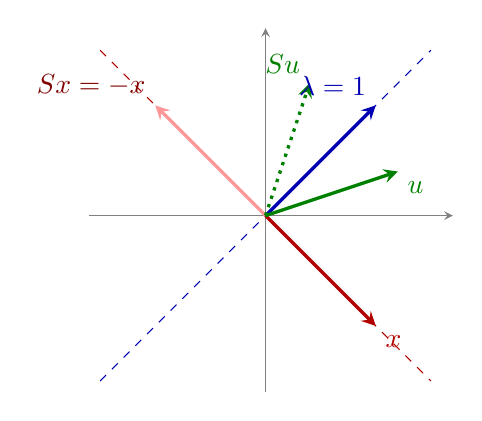
\begin{tikzpicture}[x=0.7cm,y=0.7cm,>=stealth]
  \draw[->,gray] (-3.2,0)--(3.4,0);
  \draw[->,gray] (0,-3.2)--(0,3.4);
  \draw[dashed,blue!70!black] (-3,-3)--(3,3);
  \draw[dashed,red!70!black] (-3,3)--(3,-3);
  \draw[->,very thick,blue!70!black] (0,0)--(2,2);
  \draw[->,very thick,red!70!black] (0,0)--(2,-2);
  \draw[->,very thick,red!40] (0,0)--(-2,2);
  \draw[->,very thick,green!50!black] (0,0)--(2.4,0.8);
  \draw[->,very thick,green!50!black,dotted] (0,0)--(0.8,2.4);
  \node[blue!70!black,above left] at (2,2) {$\lambda=1$};
  \node[red!70!black,below right] at (2,-2) {$x$};
  \node[red!50!black,above left] at (-2,2) {$Sx=-x$};
  \node[green!50!black,below right] at (2.4,0.8) {$u$};
  \node[green!50!black,above left] at (0.8,2.4) {$Su$};
\end{tikzpicture}
\end{center}

\noindent\textbf{Figure 2.} Reflection $S$ in the line $y=x$ (Example~\ref{ex:geom}(a)): vectors on the line are fixed (eigenvalue $1$), vectors on the dashed perpendicular line are reversed (eigenvalue $-1$), and every other vector, such as $\bv{u}$, is carried to a different line.

\subsection*{Different eigenvalues, independent eigenvectors}

Pause and think~\ref{think:sum} showed that a sum $\bv{v}+\bv{w}$ of eigenvectors for different eigenvalues is not an eigenvector. A stronger statement is true, and it is one of the main facts of this chapter.

\begin{think}{Two eigenvectors}{two}
Let $\bv{x}_1$ and $\bv{x}_2$ be eigenvectors of $A$ for $\lambda_1\neq\lambda_2$. Suppose $\bv{x}_2=c\bv{x}_1$ for some scalar $c$. (a)~Apply $A$ to both sides and compare with $\lambda_2$ times the equation. What do you get? (b)~Use this to explain why $\{\bv{x}_1,\bv{x}_2\}$ is linearly independent.
\end{think}

\begin{thm}{Eigenvectors for different eigenvalues are independent}{indep}
Let $\bv{v}_1,\dots,\bv{v}_r$ be eigenvectors of a matrix $A$ for $r$ \emph{different} eigenvalues $\lambda_1,\dots,\lambda_r$. Then $\{\bv{v}_1,\dots,\bv{v}_r\}$ is linearly independent. Consequently:
\begin{enumerate}[label=(\alph*),itemsep=1pt]
  \item an $n\times n$ matrix has at most $n$ different eigenvalues;
  \item if an $n\times n$ matrix has $n$ different eigenvalues, then eigenvectors for them form a basis of $\R^n$.
\end{enumerate}
\end{thm}

\begin{proof}
Suppose the set is dependent. A single eigenvector $\{\bv{v}_1\}$ is independent because $\bv{v}_1\neq\bv{0}$, so there is a largest $p<r$ for which $\{\bv{v}_1,\dots,\bv{v}_p\}$ is independent, and $\{\bv{v}_1,\dots,\bv{v}_{p+1}\}$ is dependent. Then some weights $c_1,\dots,c_{p+1}$, not all zero, give $c_1\bv{v}_1+\cdots+c_{p+1}\bv{v}_{p+1}=\bv{0}$. If $c_{p+1}=0$ this would be a nontrivial dependence relation among $\bv{v}_1,\dots,\bv{v}_p$, which is impossible; so $c_{p+1}\neq0$, and solving for $\bv{v}_{p+1}$ gives
\begin{equation}\label{eq:vp1}
\bv{v}_{p+1}=d_1\bv{v}_1+\cdots+d_p\bv{v}_p\qquad(d_i=-c_i/c_{p+1}).
\end{equation}
Multiply \eqref{eq:vp1} by $A$ and use $A\bv{v}_i=\lambda_i\bv{v}_i$:
\[
\lambda_{p+1}\bv{v}_{p+1}=d_1\lambda_1\bv{v}_1+\cdots+d_p\lambda_p\bv{v}_p.
\]
Multiply \eqref{eq:vp1} by $\lambda_{p+1}$ and subtract the two equations:
\[
\bv{0}=d_1(\lambda_1-\lambda_{p+1})\bv{v}_1+\cdots+d_p(\lambda_p-\lambda_{p+1})\bv{v}_p.
\]
Since $\bv{v}_1,\dots,\bv{v}_p$ are independent, every weight is zero: $d_i(\lambda_i-\lambda_{p+1})=0$. The eigenvalues are different, so $\lambda_i-\lambda_{p+1}\neq0$ and therefore $d_i=0$ for every $i$. Then \eqref{eq:vp1} says $\bv{v}_{p+1}=\bv{0}$, which contradicts the fact that an eigenvector is nonzero. Hence the set is independent.

(a)~Eigenvectors for $r$ different eigenvalues form an independent set of $r$ vectors in $\R^n$, and an independent set in $\R^n$ has at most $n$ vectors (Theorem~\ref{1.7-thm:count}), so $r\le n$. (b)~If $r=n$, we have $n$ independent vectors in the $n$-dimensional space $\R^n$, and by the Basis Theorem (Theorem~\ref{4.5-thm:basis}) they form a basis.
\end{proof}

\begin{exmp}{Three eigenvalues, three eigenvectors, one basis}{basis}
The matrix $B$ of Example~\ref{ex:test} has the eigenvalues $1$, $2$ and $4$. Eigenvectors are $\bv{v}_1=(-1,1,2)$, $\bv{v}_2=(-1,2,2)$ and $\bv{v}_3=(0,1,1)$; check: $B\bv{v}_1=(-2-1+2,\ -4+3+2,\ -4+2+4)=(-1,1,2)$, $B\bv{v}_2=(-2-2+2,\ -4+6+2,\ -4+4+4)=(-2,4,4)=2\bv{v}_2$ and $B\bv{v}_3=(-1+1,\ 3+1,\ 2+2)=(0,4,4)=4\bv{v}_3$. \ $\checkmark$ Theorem~\ref{thm:indep} says the three vectors are independent without any computation. Row reducing the matrix with these columns confirms it:
\begin{align*}
\begin{amat}{ccc}-1 & -1 & 0\\1 & 2 & 1\\2 & 2 & 1\end{amat}
&\rops{-R_1}
\begin{amat}{ccc}1 & 1 & 0\\1 & 2 & 1\\2 & 2 & 1\end{amat}
\rops{R_2-R_1,\ R_3-2R_1}
\begin{amat}{ccc}1 & 1 & 0\\0 & 1 & 1\\0 & 0 & 1\end{amat}
\\[4pt]
&\rops{R_1-R_2}
\begin{amat}{ccc}1 & 0 & -1\\0 & 1 & 1\\0 & 0 & 1\end{amat}
\rops{R_1+R_3,\ R_2-R_3}
\begin{amat}{ccc}1 & 0 & 0\\0 & 1 & 0\\0 & 0 & 1\end{amat}
\end{align*}
All three columns are pivot columns, so $\{\bv{v}_1,\bv{v}_2,\bv{v}_3\}$ is independent, and by Theorem~\ref{thm:indep}(b) it is a basis for $\R^3$. Since a $3\times3$ matrix has at most three different eigenvalues, $1$, $2$ and $4$ are \emph{all} the eigenvalues of $B$. Notice what the basis does: in the directions $\bv{v}_1,\bv{v}_2,\bv{v}_3$ the matrix $B$ simply multiplies by $1$, $2$, $4$. Writing a general vector in this basis would let us see $B\bv{x}$ at once; making that precise is what diagonalization does, in a later section.
\end{exmp}

\begin{kc}{Counting eigenvalues}{count}
(a)~Can a $3\times3$ matrix have four different eigenvalues? (b)~A $4\times4$ matrix has eigenvectors for the three different eigenvalues $1$, $2$, $3$. Are these three eigenvectors independent? Can we conclude that $\R^4$ has a basis of eigenvectors? (c)~The identity matrix $I_3$ has only one eigenvalue. Does $\R^3$ have a basis of eigenvectors of $I_3$?
\end{kc}

\subsection*{Why eigenvectors matter: powers of a matrix}

Repeated use of $A\bv{x}=\lambda\bv{x}$ gives $A^2\bv{x}=A(\lambda\bv{x})=\lambda A\bv{x}=\lambda^2\bv{x}$, then $A^3\bv{x}=\lambda^3\bv{x}$, and in general $A^k\bv{x}=\lambda^k\bv{x}$ for an eigenvector $\bv{x}$. So on an eigenvector the $k$-th power of a matrix is the $k$-th power of a \emph{number}. If a vector is a combination of eigenvectors, the same is true of every term of the combination.

\begin{exmp}{A power of a matrix applied to a vector}{powers}
Let $A=\begin{bmatrix}4&1\\2&3\end{bmatrix}$ and $\bv{x}=(5,-1)$. We know the eigenvectors $\bv{v}=(1,1)$ for $5$ and $\bv{w}=(1,-2)$ for $2$ (Example~\ref{ex:eigspaces2}). First write $\bv{x}$ as a combination of $\bv{v}$ and $\bv{w}$ by row reducing $[\,\bv{v}\ \ \bv{w}\ \ \bv{x}\,]$:
\begin{align*}
\begin{amat}{cc|c}1 & 1 & 5\\1 & -2 & -1\end{amat}
&\rops{R_2-R_1}
\begin{amat}{cc|c}1 & 1 & 5\\0 & -3 & -6\end{amat}
\rops{-\tfrac{1}{3}R_2}
\begin{amat}{cc|c}1 & 1 & 5\\0 & 1 & 2\end{amat}
\\[4pt]
&\rops{R_1-R_2}
\begin{amat}{cc|c}1 & 0 & 3\\0 & 1 & 2\end{amat}
\end{align*}
So $\bv{x}=3\bv{v}+2\bv{w}$. Then, using $A^k\bv{v}=5^k\bv{v}$ and $A^k\bv{w}=2^k\bv{w}$,
\[
A^k\bv{x}=3\cdot5^k\bv{v}+2\cdot2^k\bv{w}=\begin{bmatrix}3\cdot5^k+2\cdot2^k\\3\cdot5^k-2\cdot2^{k+1}\end{bmatrix}.
\]
For $k=3$ this is $(375+16,\ 375-32)=(391,343)$. Check by multiplying three times: $A\bv{x}=(20-1,\ 10-3)=(19,7)$, $A^2\bv{x}=(76+7,\ 38+21)=(83,59)$, $A^3\bv{x}=(332+59,\ 166+177)=(391,343)$. \ $\checkmark$ The eigenvector formula gives \emph{every} power at once and never multiplies a matrix by itself.
\end{exmp}

\begin{think}{Long-term behaviour}{powers}
(a)~In Example~\ref{ex:powers}, which of the two terms $3\cdot5^k\bv{v}$ and $2\cdot2^k\bv{w}$ is much larger when $k=20$? What does that say about the direction of $A^{20}\bv{x}$? (b)~Suppose the eigenvalues were $\tfrac12$ and $2$ instead of $5$ and $2$. What would happen to the term for $\tfrac12$ as $k$ grows?
\end{think}

\subsection*{Eigenvectors of a linear transformation}

Everything so far used only the equation $A\bv{x}=\lambda\bv{x}$, in which $A$ acts as a transformation of $\R^n$ into itself. This makes sense for any linear transformation of a vector space into itself (Section~4.2 introduced linear transformations of vector spaces).

\begin{defn}{Eigenvector of a linear transformation}{eigT}
Let $T:V\to V$ be a linear transformation of a vector space $V$ into itself. An \emph{eigenvector} of $T$ is a \emph{nonzero} vector $\bv{x}$ in $V$ such that $T(\bv{x})=\lambda\bv{x}$ for some scalar $\lambda$, which is called an \emph{eigenvalue} of $T$. The set of all $\bv{x}$ in $V$ with $T(\bv{x})=\lambda\bv{x}$ is the \emph{eigenspace} of $T$ for $\lambda$; it is a subspace of $V$ (it is the kernel of $T-\lambda\,\mathrm{id}$, and a kernel is a subspace by Theorem~\ref{4.2-thm:kersub}).
\end{defn}

For $T(\bv{x})=A\bv{x}$ on $\R^n$ this is the definition we started with. The vectors may now be polynomials, matrices or functions. Theorem~\ref{thm:indep} and its proof carry over word for word, because they use only the equation $T(\bv{x})=\lambda\bv{x}$ and linearity: eigenvectors of $T$ for different eigenvalues are independent.

\begin{exmp}{Transposing a matrix}{transpose}
Let $T:M_{2\times2}\to M_{2\times2}$ be $T(X)=X\T$, which is linear. Write $X=\begin{bmatrix}a&b\\c&d\end{bmatrix}$. Then $T(X)=\lambda X$ says
\[
\begin{bmatrix}a&c\\b&d\end{bmatrix}=\begin{bmatrix}\lambda a&\lambda b\\\lambda c&\lambda d\end{bmatrix},\qquad\text{that is}\qquad a=\lambda a,\quad c=\lambda b,\quad b=\lambda c,\quad d=\lambda d.
\]
If $\lambda=1$ the conditions reduce to $b=c$: the \emph{symmetric} matrices. So $E_1$ is the subspace of symmetric matrices, with basis $\begin{bmatrix}1&0\\0&0\end{bmatrix}$, $\begin{bmatrix}0&1\\1&0\end{bmatrix}$, $\begin{bmatrix}0&0\\0&1\end{bmatrix}$, and $\dim E_1=3$. If $\lambda=-1$ the conditions give $a=0$, $d=0$ and $c=-b$: the \emph{skew-symmetric} matrices, with basis $\begin{bmatrix}0&1\\-1&0\end{bmatrix}$ and $\dim E_{-1}=1$. No other $\lambda$ works: $c=\lambda b$ and $b=\lambda c$ give $b=\lambda^2b$, so $b=0=c$ unless $\lambda=\pm1$, and then $a=\lambda a$, $d=\lambda d$ force $a=d=0$ unless $\lambda=1$. So the eigenvalues of $T$ are exactly $1$ and $-1$.
\end{exmp}

\begin{exmp}{Differentiation}{deriv}
Let $V$ be the vector space of differentiable functions $f:\R\to\R$ and $D(f)=f'$. For every real number $\lambda$ the function $f(t)=e^{\lambda t}$ is nonzero and $D(f)=\lambda e^{\lambda t}=\lambda f$, so \emph{every} real number is an eigenvalue of $D$, with the eigenvector $e^{\lambda t}$. The eigenspace for $\lambda=2$ is $\{f:\ f'=2f\}$. If $f'=2f$, then $\bigl(e^{-2t}f\bigr)'=e^{-2t}(f'-2f)=0$, so $e^{-2t}f$ is constant and $f=ce^{2t}$. Hence $E_2=\Span\{e^{2t}\}$, of dimension $1$. Here the space is infinite-dimensional, so no matrix describes $D$, but eigenvectors still make sense.
\end{exmp}

\begin{think}{Same definition, new spaces}{newspaces}
(a)~Pick one nonzero matrix from $E_1$ and one from $E_{-1}$ in Example~\ref{ex:transpose}. Why must they be linearly independent? (The proof of Theorem~\ref{thm:indep} used only the equation $A\bv{x}=\lambda\bv{x}$ and linearity.) (b)~The dimensions of $E_1$ and $E_{-1}$ add up to $3+1=4=\dim M_{2\times2}$. What would that suggest about a basis of $M_{2\times2}$ made of eigenvectors of $T$? (c)~In Example~\ref{ex:deriv}, why can the three functions $e^{t}$, $e^{2t}$, $e^{5t}$ not be dependent?
\end{think}

\begin{kc}{Eigenvectors in a function space}{func}
Let $T:\mathbb{P}_2\to\mathbb{P}_2$ be $T(p)=tp'(t)$, where $p'$ is the derivative. (a)~Compute $T(1)$, $T(t)$ and $T(t^2)$. (b)~Find all eigenvalues of $T$ and an eigenvector for each, and say whether the eigenvectors you found are independent.
\end{kc}

\begin{kc}{True or false}{tf}
Decide whether each statement is true or false, and justify it. (a)~Every nonzero vector of $\R^n$ is an eigenvector of the identity matrix. (b)~If $A\bv{x}=\lambda\bv{x}$ for a scalar $\lambda$, then $\bv{x}$ is an eigenvector of $A$. (c)~The sum of two eigenvectors of $A$ is always an eigenvector of $A$. (d)~The eigenvalues of a triangular matrix are its diagonal entries. (e)~Every real $2\times2$ matrix has a real eigenvalue. (f)~If $A$ is invertible, then $0$ is not an eigenvalue of $A$.
\end{kc}

\subsection*{Summary}
\begin{itemize}
  \item \textbf{Definition.} An eigenvector of a square matrix $A$ is a \emph{nonzero} $\bv{x}$ with $A\bv{x}=\lambda\bv{x}$; $\lambda$ is the eigenvalue. Geometrically $\bv{x}$ stays on its line through the origin and is stretched, reversed or collapsed by the factor $\lambda$.
  \item \textbf{Testing.} To test a vector, compute $A\bv{x}$ and compare it with $\bv{x}$. To test a scalar, row reduce $[\,A-\lambda I\ \ \bv{0}\,]$: $\lambda$ is an eigenvalue exactly when there is a free variable (Theorem~\ref{thm:test}).
  \item \textbf{Eigenspace.} $E_\lambda=\Nul(A-\lambda I)$ is a subspace; a basis comes from the free variables (Procedure~\ref{proc:eigspace}), and $\dim E_\lambda$ is their number. Only eigenvectors for the \emph{same} eigenvalue may be combined.
  \item \textbf{Special cases.} $0$ is an eigenvalue exactly when $A$ is not invertible, and $E_0=\Nul A$. The eigenvalues of a triangular matrix are its diagonal entries; a repeated diagonal entry does not guarantee a two-dimensional eigenspace (Example~\ref{ex:tri}).
  \item \textbf{Independence.} Eigenvectors for different eigenvalues are linearly independent (Theorem~\ref{thm:indep}). So an $n\times n$ matrix has at most $n$ eigenvalues, and with $n$ different eigenvalues the eigenvectors form a basis of $\R^n$.
  \item \textbf{Other spaces.} A linear transformation $T:V\to V$ has eigenvectors and eigenvalues too (Definition~\ref{def:eigT}): symmetric and skew-symmetric matrices for $X\mapsto X\T$, exponentials for differentiation.
\end{itemize}

\subsection*{Questions to think about}
\begin{enumerate}
  \item Let $A$ be a $2\times2$ matrix for which \emph{every} nonzero vector of $\R^2$ is an eigenvector. Show that $A=\lambda I$ for a single scalar $\lambda$. (Look at $\bv{e}_1$, $\bv{e}_2$ and $\bv{e}_1+\bv{e}_2$.)
  \item Describe the eigenvalues and eigenspaces of the zero matrix and of the identity matrix. How do they differ from those of $2I$?
  \item Let $T:\mathbb{P}_2\to\mathbb{P}_2$ be $T(p)(t)=p(-t)$. Find the eigenvalues and describe the eigenspaces. Which one has dimension $2$?
\end{enumerate}

\subsection*{Example bank}
The twelve examples below add problem types that the worked examples above do not cover: testing vectors and scalars on new matrices, eigenspaces of dimension two in $3\times3$ and $4\times4$ matrices, a parameter that decides the dimension of an eigenspace, eigenvalues that can be seen without any row reduction, an operator on polynomials with a single eigenvalue, and three proofs. Within each group the examples go from easier to harder. Work each problem before you read its solution.

\textbf{What is in this bank.}
\begin{itemize}
  \item \textbf{Bank A, testing a vector or a scalar:} Example~\ref{ex:b-testvec} (which vectors are eigenvectors), Example~\ref{ex:b-testscalar} (which scalars are eigenvalues, with eigenspaces) and Example~\ref{ex:b-unknown} (an unknown entry fixed by an eigenvector).
  \item \textbf{Bank B, eigenspaces of dimension two:} Example~\ref{ex:b-plane3} (a $3\times3$ matrix), Example~\ref{ex:b-four4} (a $4\times4$ matrix) and Example~\ref{ex:b-dimh} (a parameter $h$ decides $\dim E_2$).
  \item \textbf{Bank C, eigenvalues you can see:} Example~\ref{ex:b-rowsum} (constant row sums and a rank-one matrix) and Example~\ref{ex:b-triparam} (a triangular matrix with a parameter).
  \item \textbf{Bank D, another space:} Example~\ref{ex:b-diffop} (a difference operator on $\mathbb{P}_2$ with one eigenvalue).
  \item \textbf{Bank E, proofs:} Example~\ref{ex:b-psquare} (beginner: eigenvalues of $A^2$), Example~\ref{ex:b-inverse} (intermediate: eigenvalues of $A^{-1}$) and Example~\ref{ex:b-sumnot} (intermediate: a sum of eigenvectors).
\end{itemize}

\subsection*{Bank A: Testing a vector or a scalar}
\begin{exmp}{Which vectors are eigenvectors?}{b-testvec}
Let $M=\begin{bmatrix}5&-6\\3&-4\end{bmatrix}$. For each of $\bv{a}=(4,2)$, $\bv{b}=(-3,-3)$ and $\bv{c}=(1,2)$, decide whether it is an eigenvector of $M$, and give the eigenvalue if it is.

\textbf{Solution.} Multiply, then ask whether the result is a multiple of the vector you started with.
\[
M\bv{a}=\begin{bmatrix}20-12\\12-8\end{bmatrix}=\begin{bmatrix}8\\4\end{bmatrix}=2\bv{a},\qquad
M\bv{b}=\begin{bmatrix}-15+18\\-9+12\end{bmatrix}=\begin{bmatrix}3\\3\end{bmatrix}=-1\cdot\bv{b},\qquad
M\bv{c}=\begin{bmatrix}5-12\\3-8\end{bmatrix}=\begin{bmatrix}-7\\-5\end{bmatrix}.
\]
So $\bv{a}$ is an eigenvector for $2$, and $\bv{b}$ is an eigenvector for $-1$. For $\bv{c}$, a multiple $\lambda(1,2)$ would have second entry twice the first, but $-5\neq2(-7)$, so $\bv{c}$ is not an eigenvector. Notice that $\bv{a}=(4,2)$ is a multiple of $(2,1)$: the eigenvector is a whole line, and any nonzero multiple of an eigenvector is again one.
\end{exmp}

\begin{exmp}{Which scalars are eigenvalues, and what are their eigenspaces?}{b-testscalar}
Let $A=\begin{bmatrix}1&-3&0\\0&-2&0\\-4&4&3\end{bmatrix}$. Decide whether $3$, $2$ and $-2$ are eigenvalues of $A$, and for each eigenvalue find a basis for its eigenspace.

\textbf{Solution.} A scalar $\lambda$ is an eigenvalue exactly when $(A-\lambda I)\bv{x}=\bv{0}$ has a free variable (Theorem~\ref{thm:test}), so we row reduce $[\,A-\lambda I\ \ \bv{0}\,]$ for each. For $\lambda=3$:
\begin{align*}
\begin{amat}{ccc|c}-2 & -3 & 0 & 0\\0 & -5 & 0 & 0\\-4 & 4 & 0 & 0\end{amat}
&\rops{-\tfrac{1}{2}R_1}
\begin{amat}{ccc|c}1 & \tfrac{3}{2} & 0 & 0\\0 & -5 & 0 & 0\\-4 & 4 & 0 & 0\end{amat}
\rops{R_3+4R_1}
\begin{amat}{ccc|c}1 & \tfrac{3}{2} & 0 & 0\\0 & -5 & 0 & 0\\0 & 10 & 0 & 0\end{amat}
\\[4pt]
&\rops{-\tfrac{1}{5}R_2}
\begin{amat}{ccc|c}1 & \tfrac{3}{2} & 0 & 0\\0 & 1 & 0 & 0\\0 & 10 & 0 & 0\end{amat}
\rops{R_1-\tfrac{3}{2}R_2,\ R_3-10R_2}
\begin{amat}{ccc|c}1 & 0 & 0 & 0\\0 & 1 & 0 & 0\\0 & 0 & 0 & 0\end{amat}
\end{align*}
$x_3$ is free and $x_1=x_2=0$, so $3$ is an eigenvalue and $E_3=\Span\{(0,0,1)\}$. For $\lambda=2$:
\begin{align*}
\begin{amat}{ccc|c}-1 & -3 & 0 & 0\\0 & -4 & 0 & 0\\-4 & 4 & 1 & 0\end{amat}
&\rops{-R_1}
\begin{amat}{ccc|c}1 & 3 & 0 & 0\\0 & -4 & 0 & 0\\-4 & 4 & 1 & 0\end{amat}
\rops{R_3+4R_1}
\begin{amat}{ccc|c}1 & 3 & 0 & 0\\0 & -4 & 0 & 0\\0 & 16 & 1 & 0\end{amat}
\\[4pt]
&\rops{-\tfrac{1}{4}R_2}
\begin{amat}{ccc|c}1 & 3 & 0 & 0\\0 & 1 & 0 & 0\\0 & 16 & 1 & 0\end{amat}
\rops{R_1-3R_2,\ R_3-16R_2}
\begin{amat}{ccc|c}1 & 0 & 0 & 0\\0 & 1 & 0 & 0\\0 & 0 & 1 & 0\end{amat}
\end{align*}
Every column has a pivot, so $2$ is \emph{not} an eigenvalue. For $\lambda=-2$:
\begin{align*}
\begin{amat}{ccc|c}3 & -3 & 0 & 0\\0 & 0 & 0 & 0\\-4 & 4 & 5 & 0\end{amat}
&\rops{\tfrac{1}{3}R_1}
\begin{amat}{ccc|c}1 & -1 & 0 & 0\\0 & 0 & 0 & 0\\-4 & 4 & 5 & 0\end{amat}
\rops{R_3+4R_1}
\begin{amat}{ccc|c}1 & -1 & 0 & 0\\0 & 0 & 0 & 0\\0 & 0 & 5 & 0\end{amat}
\\[4pt]
&\rops{R_2\leftrightarrow R_3}
\begin{amat}{ccc|c}1 & -1 & 0 & 0\\0 & 0 & 5 & 0\\0 & 0 & 0 & 0\end{amat}
\rops{\tfrac{1}{5}R_2}
\begin{amat}{ccc|c}1 & -1 & 0 & 0\\0 & 0 & 1 & 0\\0 & 0 & 0 & 0\end{amat}
\end{align*}
Here $x_2$ is free, with $x_1=x_2$ and $x_3=0$. So $-2$ is an eigenvalue and $E_{-2}=\Span\{(1,1,0)\}$. Check: $A(1,1,0)=(1-3,\ -2,\ -4+4)=(-2,-2,0)=-2(1,1,0)$. \ $\checkmark$
\end{exmp}

\begin{exmp}{An unknown entry}{b-unknown}
The vector $\bv{x}=(1,2)$ is an eigenvector of $M_h=\begin{bmatrix}1&h\\4&1\end{bmatrix}$. Find $h$ and the eigenvalue. Then find the other eigenvalue of $M_h$ and an eigenvector for it.

\textbf{Solution.} If $\bv{x}$ is an eigenvector, then $M_h\bv{x}=\lambda\bv{x}$ for some $\lambda$. Compute
\[
M_h\bv{x}=\begin{bmatrix}1+2h\\4+2\end{bmatrix}=\begin{bmatrix}1+2h\\6\end{bmatrix}=\lambda\begin{bmatrix}1\\2\end{bmatrix}.
\]
The second entry gives $2\lambda=6$, so $\lambda=3$ (the entry that does not involve $h$ is the one to use first). The first entry then gives $1+2h=3$, so $h=1$. Now $M_1=\begin{bmatrix}1&1\\4&1\end{bmatrix}$. Row reduce $[\,M_1-\lambda I\ \ \bv{0}\,]$ for a second eigenvalue; looking at the matrix, try $\lambda=-1$:
\begin{align*}
\begin{amat}{cc|c}2 & 1 & 0\\4 & 2 & 0\end{amat}
&\rops{\tfrac{1}{2}R_1}
\begin{amat}{cc|c}1 & \tfrac{1}{2} & 0\\4 & 2 & 0\end{amat}
\rops{R_2-4R_1}
\begin{amat}{cc|c}1 & \tfrac{1}{2} & 0\\0 & 0 & 0\end{amat}
\end{align*}
There is a free variable, so $-1$ is an eigenvalue, with $x_1=-\tfrac12x_2$; taking $x_2=-2$ gives the eigenvector $(1,-2)$. Check: $M_1(1,-2)=(1-2,\ 4-2)=(-1,2)=-1\cdot(1,-2)$. \ $\checkmark$ By Theorem~\ref{thm:indep}(a) a $2\times2$ matrix has at most two eigenvalues, so $3$ and $-1$ are all of them.
\end{exmp}

\subsection*{Bank B: Eigenspaces of dimension two}
\begin{exmp}{A $3\times3$ matrix with a two-dimensional eigenspace}{b-plane3}
Let $A=\begin{bmatrix}5&3&-3\\-3&-1&3\\-3&-3&5\end{bmatrix}$. Show that $2$ and $5$ are eigenvalues, and find a basis for each eigenspace.

\textbf{Solution.} For $\lambda=2$:
\begin{align*}
\begin{amat}{ccc|c}3 & 3 & -3 & 0\\-3 & -3 & 3 & 0\\-3 & -3 & 3 & 0\end{amat}
&\rops{\tfrac{1}{3}R_1}
\begin{amat}{ccc|c}1 & 1 & -1 & 0\\-3 & -3 & 3 & 0\\-3 & -3 & 3 & 0\end{amat}
\rops{R_2+3R_1,\ R_3+3R_1}
\begin{amat}{ccc|c}1 & 1 & -1 & 0\\0 & 0 & 0 & 0\\0 & 0 & 0 & 0\end{amat}
\end{align*}
$x_2$ and $x_3$ are free and $x_1=-x_2+x_3$, so
\[
\bv{x}=x_2\begin{bmatrix}-1\\1\\0\end{bmatrix}+x_3\begin{bmatrix}1\\0\\1\end{bmatrix},
\]
and $\{(-1,1,0),(1,0,1)\}$ is a basis for $E_2$; $\dim E_2=2$. For $\lambda=5$:
\begin{align*}
\begin{amat}{ccc|c}0 & 3 & -3 & 0\\-3 & -6 & 3 & 0\\-3 & -3 & 0 & 0\end{amat}
&\rops{R_1\leftrightarrow R_2}
\begin{amat}{ccc|c}-3 & -6 & 3 & 0\\0 & 3 & -3 & 0\\-3 & -3 & 0 & 0\end{amat}
\rops{-\tfrac{1}{3}R_1}
\begin{amat}{ccc|c}1 & 2 & -1 & 0\\0 & 3 & -3 & 0\\-3 & -3 & 0 & 0\end{amat}
\\[4pt]
&\rops{R_3+3R_1}
\begin{amat}{ccc|c}1 & 2 & -1 & 0\\0 & 3 & -3 & 0\\0 & 3 & -3 & 0\end{amat}
\rops{\tfrac{1}{3}R_2}
\begin{amat}{ccc|c}1 & 2 & -1 & 0\\0 & 1 & -1 & 0\\0 & 3 & -3 & 0\end{amat}
\\[4pt]
&\rops{R_1-2R_2,\ R_3-3R_2}
\begin{amat}{ccc|c}1 & 0 & 1 & 0\\0 & 1 & -1 & 0\\0 & 0 & 0 & 0\end{amat}
\end{align*}
$x_3$ is free, $x_1=-x_3$ and $x_2=x_3$, so $E_5=\Span\{(-1,1,1)\}$. Check: $A(-1,1,0)=(-5+3,\ 3-1,\ 3-3)=(-2,2,0)=2(-1,1,0)$; $A(1,0,1)=(5-3,\ -3+3,\ -3+5)=(2,0,2)=2(1,0,1)$; $A(-1,1,1)=(-5+3-3,\ 3-1+3,\ 3-3+5)=(-5,5,5)=5(-1,1,1)$. \ $\checkmark$ The three basis vectors together are independent (they come from different eigenspaces), so they form a basis of $\R^3$ made of eigenvectors, even though $A$ has only two different eigenvalues.
\end{exmp}

\begin{exmp}{The eigenspace of a $4\times4$ matrix}{b-four4}
Let $A=\begin{bmatrix}2&1&-1&-1\\0&1&1&1\\-3&-5&4&5\\3&3&0&-1\end{bmatrix}$. Find a basis for the eigenspace $E_2$ and give $\dim E_2$.

\textbf{Solution.} Row reduce $[\,A-2I\ \ \bv{0}\,]$, where $A-2I$ has diagonal entries $0,-1,2,-3$:
\begin{align*}
\begin{amat}{cccc|c}0 & 1 & -1 & -1 & 0\\0 & -1 & 1 & 1 & 0\\-3 & -5 & 2 & 5 & 0\\3 & 3 & 0 & -3 & 0\end{amat}
&\rops{R_2+R_1,\ R_4+R_3}
\begin{amat}{cccc|c}0 & 1 & -1 & -1 & 0\\0 & 0 & 0 & 0 & 0\\-3 & -5 & 2 & 5 & 0\\0 & -2 & 2 & 2 & 0\end{amat}
\rops{R_4+2R_1}
\begin{amat}{cccc|c}0 & 1 & -1 & -1 & 0\\0 & 0 & 0 & 0 & 0\\-3 & -5 & 2 & 5 & 0\\0 & 0 & 0 & 0 & 0\end{amat}
\\[4pt]
&\rops{R_3+5R_1}
\begin{amat}{cccc|c}0 & 1 & -1 & -1 & 0\\0 & 0 & 0 & 0 & 0\\-3 & 0 & -3 & 0 & 0\\0 & 0 & 0 & 0 & 0\end{amat}
\rops{R_1\leftrightarrow R_3}
\begin{amat}{cccc|c}-3 & 0 & -3 & 0 & 0\\0 & 0 & 0 & 0 & 0\\0 & 1 & -1 & -1 & 0\\0 & 0 & 0 & 0 & 0\end{amat}
\\[4pt]
&\rops{-\tfrac{1}{3}R_1}
\begin{amat}{cccc|c}1 & 0 & 1 & 0 & 0\\0 & 0 & 0 & 0 & 0\\0 & 1 & -1 & -1 & 0\\0 & 0 & 0 & 0 & 0\end{amat}
\rops{R_2\leftrightarrow R_3}
\begin{amat}{cccc|c}1 & 0 & 1 & 0 & 0\\0 & 1 & -1 & -1 & 0\\0 & 0 & 0 & 0 & 0\\0 & 0 & 0 & 0 & 0\end{amat}
\end{align*}
The variables $x_3$ and $x_4$ are free, with $x_1=-x_3$ and $x_2=x_3+x_4$. Hence
\[
\bv{x}=x_3\begin{bmatrix}-1\\1\\1\\0\end{bmatrix}+x_4\begin{bmatrix}0\\1\\0\\1\end{bmatrix},
\]
and $\{(-1,1,1,0),(0,1,0,1)\}$ is a basis for $E_2$, so $\dim E_2=2$. Check: $A(-1,1,1,0)=(-2+1-1,\ 1+1,\ 3-5+4,\ -3+3)=(-2,2,2,0)=2(-1,1,1,0)$ and $A(0,1,0,1)=(1-1,\ 1+1,\ -5+5,\ 3-1)=(0,2,0,2)=2(0,1,0,1)$. \ $\checkmark$ Two rows of $A-2I$ are negatives of each other (rows $1$ and $2$), which is why the rank dropped to $2$; this is the kind of coincidence to look for.
\end{exmp}

\begin{exmp}{A parameter decides the dimension of an eigenspace}{b-dimh}
Let $G_h=\begin{bmatrix}2&h&0\\0&2&0\\1&0&5\end{bmatrix}$. The number $2$ is an eigenvalue of $G_h$ for every $h$. For which $h$ is $\dim E_2=2$, and for which $h$ is $\dim E_2=1$? Find a basis for $E_2$ in each case.

\textbf{Solution.} We must count the free variables of $(G_h-2I)\bv{x}=\bv{0}$, so row reduce $[\,G_h-2I\ \ \bv{0}\,]$:
\begin{align*}
\begin{amat}{ccc|c}0 & h & 0 & 0\\0 & 0 & 0 & 0\\1 & 0 & 3 & 0\end{amat}
&\rops{R_1\leftrightarrow R_3}
\begin{amat}{ccc|c}1 & 0 & 3 & 0\\0 & 0 & 0 & 0\\0 & h & 0 & 0\end{amat}
\rops{R_2\leftrightarrow R_3}
\begin{amat}{ccc|c}1 & 0 & 3 & 0\\0 & h & 0 & 0\\0 & 0 & 0 & 0\end{amat}
\end{align*}
\emph{Case $h\neq0$.} The row $(0,h,0\mid0)$ has a pivot in column $2$, so there are pivots in columns $1$ and $2$ and one free variable, $x_3$. Then $x_2=0$ and $x_1=-3x_3$, so $\dim E_2=1$ and $E_2=\Span\{(-3,0,1)\}$. Check: $G_h(-3,0,1)=(-6,\ 0,\ -3+5)=(-6,0,2)=2(-3,0,1)$. \ $\checkmark$

\emph{Case $h=0$.} The second row is zero, so only column $1$ has a pivot, $x_2$ and $x_3$ are free, $x_1=-3x_3$ and
\[
\bv{x}=x_2\begin{bmatrix}0\\1\\0\end{bmatrix}+x_3\begin{bmatrix}-3\\0\\1\end{bmatrix},
\]
so $\dim E_2=2$. Check the new vector: $G_0(0,1,0)=(0,2,0)=2(0,1,0)$. \ $\checkmark$ (For $h\neq0$ the same vector gives $G_h(0,1,0)=(h,2,0)$, which is not a multiple of $(0,1,0)$.) So one eigenvalue can have a one-dimensional or a two-dimensional eigenspace, depending on a single entry of the matrix.
\end{exmp}

\subsection*{Bank C: Eigenvalues you can see}
\begin{exmp}{Constant row sums and a rank-one matrix}{b-rowsum}
(a)~Show that $5$ is an eigenvalue of $M=\begin{bmatrix}2&1&2\\3&0&2\\1&3&1\end{bmatrix}$ without row reducing. (b)~Find the eigenvalues of $N=\begin{bmatrix}2&4\\1&2\end{bmatrix}$ and an eigenvector for each.

\textbf{Solution.} (a)~Every row of $M$ adds up to $5$. Multiplying $M$ by $(1,1,1)$ adds each row, so
\[
M\begin{bmatrix}1\\1\\1\end{bmatrix}=\begin{bmatrix}2+1+2\\3+0+2\\1+3+1\end{bmatrix}=\begin{bmatrix}5\\5\\5\end{bmatrix}=5\begin{bmatrix}1\\1\\1\end{bmatrix}.
\]
So $(1,1,1)$ is an eigenvector for $5$.

(b)~The first row of $N$ is twice the second row, so $N$ is not invertible and $0$ is an eigenvalue (Theorem~\ref{thm:test}). Its eigenspace is $\Nul N$: $2x_1+4x_2=0$ gives $x_1=-2x_2$, so $(-2,1)$ is an eigenvector. For the other eigenvalue, notice that both columns of $N$ are multiples of $(2,1)$, so $N\bv{x}$ always lies on the line through $(2,1)$; in particular $N(2,1)=(4+4,\ 2+2)=(8,4)=4(2,1)$. So $4$ is an eigenvalue with the eigenvector $(2,1)$. A $2\times2$ matrix has at most two eigenvalues (Theorem~\ref{thm:indep}), so $0$ and $4$ are all of them.
\end{exmp}

\begin{exmp}{A triangular matrix with a parameter}{b-triparam}
Let $T_c=\begin{bmatrix}c&1&0\\0&2&5\\0&0&c-3\end{bmatrix}$. (a)~Find the eigenvalues of $T_c$. (b)~For which $c$ is $T_c$ not invertible? (c)~For which $c$ does $T_c$ have fewer than three different eigenvalues?

\textbf{Solution.} (a)~$T_c$ is triangular, so by Theorem~\ref{thm:tri} its eigenvalues are the diagonal entries $c$, $2$ and $c-3$.

(b)~$T_c$ fails to be invertible exactly when $0$ is an eigenvalue (Theorem~\ref{thm:test}), that is, when one of $c$, $2$, $c-3$ equals $0$. The entry $2$ never does, so $T_c$ is singular exactly for $c=0$ and $c=3$.

(c)~There are fewer than three different eigenvalues exactly when two of the three diagonal entries coincide. The first entry equals the second when $c=2$; the third equals the second when $c-3=2$, that is $c=5$; and $c=c-3$ never holds. So the eigenvalues are three different numbers except for $c=2$ (eigenvalues $2,2,-1$) and $c=5$ (eigenvalues $5,2,2$). For $c=2$ the eigenvalue $2$ appears twice, but $E_2$ is one-dimensional: $T_2-2I=\begin{bmatrix}0&1&0\\0&0&5\\0&0&-3\end{bmatrix}$ has pivots in columns $2$ and $3$, so only $x_1$ is free.
\end{exmp}

\subsection*{Bank D: Another space}
\begin{exmp}{An operator with only one eigenvalue}{b-diffop}
Let $\Delta:\mathbb{P}_2\to\mathbb{P}_2$ be $\Delta(p)(t)=p(t+1)-p(t)$, which is linear. Find all eigenvalues and eigenspaces of $\Delta$.

\textbf{Solution.} Write $p=a+bt+ct^2$. Then $p(t+1)=a+b(t+1)+c(t+1)^2=(a+b+c)+(b+2c)t+ct^2$, so
\[
\Delta(p)=(b+c)+2c\,t+0\,t^2.
\]
The equation $\Delta(p)=\lambda p$ says, coefficient by coefficient,
\[
b+c=\lambda a,\qquad 2c=\lambda b,\qquad 0=\lambda c.
\]
\emph{If $\lambda\neq0$:} the last equation gives $c=0$, then $2c=\lambda b$ gives $b=0$, then $b+c=\lambda a$ gives $a=0$, so $p=0$ and $\lambda$ is not an eigenvalue. \emph{If $\lambda=0$:} the equations become $b+c=0$, $2c=0$, so $c=0$, $b=0$ and $a$ is free. Hence the only eigenvalue is $0$, and $E_0=\Span\{1\}$, the constant polynomials (indeed $\Delta(1)=1-1=0$). Unlike $\R^2$ with a rotation, there is an eigenvalue here, but there are far fewer eigenvectors than $\dim\mathbb{P}_2=3$: the eigenvectors do not come near to forming a basis of $\mathbb{P}_2$.
\end{exmp}

\subsection*{Bank E: Proofs}
\begin{exmp}{The eigenvalues of $A^2$}{b-psquare}
\textbf{Statement.} Let $A$ be an $n\times n$ matrix. If $\lambda$ is an eigenvalue of $A$ with eigenvector $\bv{x}$, then $\lambda^2$ is an eigenvalue of $A^2$, and $\bv{x}$ is an eigenvector of $A^2$ for $\lambda^2$.

\textbf{Plan.} We must produce a nonzero vector $\bv{y}$ with $A^2\bv{y}=\lambda^2\bv{y}$. The only information is $A\bv{x}=\lambda\bv{x}$ with $\bv{x}\neq\bv{0}$, so try $\bv{y}=\bv{x}$ and use the information twice.

\textbf{Proof.}
\emph{Step 1 (unwind $A^2$).} By definition of the power, $A^2\bv{x}=A(A\bv{x})$.
\emph{Step 2 (use the hypothesis once).} Since $A\bv{x}=\lambda\bv{x}$, we get $A(A\bv{x})=A(\lambda\bv{x})$.
\emph{Step 3 (pull out the scalar).} By linearity of matrix multiplication (Theorem~\ref{1.4-thm:linear}), $A(\lambda\bv{x})=\lambda A\bv{x}$.
\emph{Step 4 (use the hypothesis again).} $\lambda A\bv{x}=\lambda(\lambda\bv{x})=\lambda^2\bv{x}$.
Combining the four steps, $A^2\bv{x}=\lambda^2\bv{x}$ with $\bv{x}\neq\bv{0}$, which says that $\bv{x}$ is an eigenvector of $A^2$ for the eigenvalue $\lambda^2$. \qquad$\blacksquare$

\textbf{Common mistake.} Reading the statement backwards. It does \emph{not} say that every eigenvalue of $A^2$ comes from an eigenvalue of $A$. The rotation $R=\begin{bmatrix}0&-1\\1&0\end{bmatrix}$ of Example~\ref{ex:geom} has no real eigenvalue, yet $R^2=-I$ has the eigenvalue $-1$ (every nonzero vector is an eigenvector). A second mistake is to forget $\bv{x}\neq\bv{0}$: the equation $A^2\bv{x}=\lambda^2\bv{x}$ holds for $\bv{x}=\bv{0}$ whatever $\lambda$ is, so the hypothesis that $\bv{x}$ is an eigenvector is what makes the conclusion meaningful. Numerical check with $A=\begin{bmatrix}4&1\\2&3\end{bmatrix}$, $\bv{x}=(1,1)$, $\lambda=5$: $A^2=\begin{bmatrix}18&7\\14&11\end{bmatrix}$ and $A^2\bv{x}=(25,25)=25\bv{x}$.
\end{exmp}

\begin{exmp}{The eigenvalues of $A^{-1}$}{b-inverse}
\textbf{Statement.} Let $A$ be an invertible $n\times n$ matrix and let $\bv{x}$ be an eigenvector of $A$ for the eigenvalue $\lambda$. Then $\lambda\neq0$, and $\bv{x}$ is an eigenvector of $A^{-1}$ for the eigenvalue $1/\lambda$.

\textbf{Plan.} Two things must be shown: that $\lambda$ can be divided by, and that $A^{-1}\bv{x}=\frac{1}{\lambda}\bv{x}$. For the first we need to know when $0$ is an eigenvalue (Theorem~\ref{thm:test}). For the second, the inverse undoes $A$, so apply $A^{-1}$ to the equation $A\bv{x}=\lambda\bv{x}$.

\textbf{Proof.}
\emph{Step 1 ($\lambda\neq0$).} By Theorem~\ref{thm:test}, $0$ is an eigenvalue of a matrix if and only if the matrix is not invertible. $A$ is invertible, so $0$ is not an eigenvalue of $A$. Since $\lambda$ is an eigenvalue, $\lambda\neq0$.
\emph{Step 2 (apply the inverse).} Multiply $A\bv{x}=\lambda\bv{x}$ on the left by $A^{-1}$: $A^{-1}(A\bv{x})=A^{-1}(\lambda\bv{x})$.
\emph{Step 3 (simplify both sides).} The left side is $(A^{-1}A)\bv{x}=I\bv{x}=\bv{x}$. On the right, linearity (Theorem~\ref{1.4-thm:linear}) gives $A^{-1}(\lambda\bv{x})=\lambda A^{-1}\bv{x}$. So $\bv{x}=\lambda A^{-1}\bv{x}$.
\emph{Step 4 (divide by $\lambda$).} This step is allowed by Step 1: $A^{-1}\bv{x}=\frac{1}{\lambda}\bv{x}$. Since $\bv{x}\neq\bv{0}$, it is an eigenvector of $A^{-1}$ for $1/\lambda$. \qquad$\blacksquare$

\textbf{Common mistake.} Dividing by $\lambda$ in Step 4 without having shown $\lambda\neq0$. The hypothesis ``$A$ is invertible'' is used exactly once, in Step 1 (and implicitly to have $A^{-1}$ at all). Numerical check with $A=\begin{bmatrix}4&1\\2&3\end{bmatrix}$, $\bv{x}=(1,-2)$, $\lambda=2$: $A^{-1}=\tfrac{1}{10}\begin{bmatrix}3&-1\\-2&4\end{bmatrix}$ and $A^{-1}\bv{x}=\tfrac{1}{10}(5,-10)=(\tfrac12,-1)=\tfrac12\bv{x}$.
\end{exmp}

\begin{exmp}{A sum of eigenvectors is usually not an eigenvector}{b-sumnot}
\textbf{Statement.} Let $\bv{x}$ and $\bv{y}$ be eigenvectors of $A$ for two \emph{different} eigenvalues $\lambda$ and $\mu$. Then $\bv{x}+\bv{y}$ is not an eigenvector of $A$.

\textbf{Plan.} Assume the opposite, that $\bv{x}+\bv{y}$ is an eigenvector for some $\nu$, and look for a contradiction. The assumption gives an equation among $\bv{x}$ and $\bv{y}$; Theorem~\ref{thm:indep} says that $\bv{x}$ and $\bv{y}$ are independent, so the weights in that equation must vanish.

\textbf{Proof.}
\emph{Step 1 (assume the opposite).} Suppose $A(\bv{x}+\bv{y})=\nu(\bv{x}+\bv{y})$ for some scalar $\nu$.
\emph{Step 2 (expand the left side).} By linearity, $A(\bv{x}+\bv{y})=A\bv{x}+A\bv{y}=\lambda\bv{x}+\mu\bv{y}$.
\emph{Step 3 (collect).} Comparing the two sides, $\lambda\bv{x}+\mu\bv{y}=\nu\bv{x}+\nu\bv{y}$, that is, $(\lambda-\nu)\bv{x}+(\mu-\nu)\bv{y}=\bv{0}$.
\emph{Step 4 (use independence).} The vectors $\bv{x}$ and $\bv{y}$ are eigenvectors for different eigenvalues, so they are linearly independent (Theorem~\ref{thm:indep}). Hence both weights are zero: $\lambda-\nu=0$ and $\mu-\nu=0$.
\emph{Step 5 (contradiction).} Then $\lambda=\nu=\mu$, which contradicts $\lambda\neq\mu$. So no such $\nu$ exists. \qquad$\blacksquare$

\textbf{Common mistake.} Using ``the sum of two eigenvectors is an eigenvector'' from Theorem~\ref{thm:eigsub}. That theorem is about eigenvectors for the \emph{same} eigenvalue. Check that the hypothesis ``different eigenvalues'' is really used: it enters in Step 4 (independence) and in Step 5. If $\lambda=\mu$ the statement is false, because then $\bv{x}+\bv{y}$ is an eigenvector for $\lambda$ (when it is nonzero). Numerical check with $A=\begin{bmatrix}4&1\\2&3\end{bmatrix}$: $\bv{x}=(1,1)$ and $\bv{y}=(1,-2)$ give $A(\bv{x}+\bv{y})=A(2,-1)=(7,1)$, which is not a multiple of $(2,-1)$.
\end{exmp}

\subsection*{Answers and discussion}
\begin{description}[leftmargin=0pt,itemsep=5pt]
  \item[Knowledge Check \ref{kc:vec}.] (a)~$A(1,1)=(3-2,\ 1)=(1,1)$: an eigenvector for $\lambda=1$. (b)~$A(2,1)=(6-2,\ 2)=(4,2)=2(2,1)$: an eigenvector for $\lambda=2$. (c)~$A(1,2)=(3-4,\ 1)=(-1,1)$, not a multiple of $(1,2)$: not an eigenvector. (d)~$A(-4,-2)=(-12+4,\ -4)=(-8,-4)=2(-4,-2)$: an eigenvector for $\lambda=2$ (it is a multiple of the vector in (b)).
  \item[Knowledge Check \ref{kc:scalar}.] (a)~Row reduce $[\,A-4I\ \ \bv{0}\,]$:
\begin{align*}
\begin{amat}{cc|c}-3 & 2 & 0\\3 & -2 & 0\end{amat}
&\rops{-\tfrac{1}{3}R_1}
\begin{amat}{cc|c}1 & -\tfrac{2}{3} & 0\\3 & -2 & 0\end{amat}
\rops{R_2-3R_1}
\begin{amat}{cc|c}1 & -\tfrac{2}{3} & 0\\0 & 0 & 0\end{amat}
\end{align*}
  $x_2$ is free, $x_1=\tfrac23x_2$; with $x_2=3$ we get the eigenvector $(2,3)$, so $4$ is an eigenvalue. Check: $A(2,3)=(2+6,\ 6+6)=(8,12)=4(2,3)$. \ $\checkmark$ (b)~Row reduce $[\,A-2I\ \ \bv{0}\,]$:
\begin{align*}
\begin{amat}{cc|c}-1 & 2 & 0\\3 & 0 & 0\end{amat}
&\rops{-R_1}
\begin{amat}{cc|c}1 & -2 & 0\\3 & 0 & 0\end{amat}
\rops{R_2-3R_1}
\begin{amat}{cc|c}1 & -2 & 0\\0 & 6 & 0\end{amat}
\\[4pt]
&\rops{\tfrac{1}{6}R_2}
\begin{amat}{cc|c}1 & -2 & 0\\0 & 1 & 0\end{amat}
\rops{R_1+2R_2}
\begin{amat}{cc|c}1 & 0 & 0\\0 & 1 & 0\end{amat}
\end{align*}
  Both columns have pivots, so $2$ is not an eigenvalue. (c)~$0$ is an eigenvalue exactly when $A$ is not invertible (Theorem~\ref{thm:test}). Here $\det A=1\cdot2-2\cdot3=-4\neq0$, so $A$ is invertible (Theorem~\ref{2.2-thm:twobytwo}) and $0$ is not an eigenvalue.
  \item[Knowledge Check \ref{kc:space}.] (a)~$A-2I=\begin{bmatrix}0&0&0\\1&0&0\\0&0&3\end{bmatrix}$:
\begin{align*}
\begin{amat}{ccc|c}0 & 0 & 0 & 0\\1 & 0 & 0 & 0\\0 & 0 & 3 & 0\end{amat}
&\rops{R_1\leftrightarrow R_2}
\begin{amat}{ccc|c}1 & 0 & 0 & 0\\0 & 0 & 0 & 0\\0 & 0 & 3 & 0\end{amat}
\rops{R_2\leftrightarrow R_3}
\begin{amat}{ccc|c}1 & 0 & 0 & 0\\0 & 0 & 3 & 0\\0 & 0 & 0 & 0\end{amat}
\\[4pt]
&\rops{\tfrac{1}{3}R_2}
\begin{amat}{ccc|c}1 & 0 & 0 & 0\\0 & 0 & 1 & 0\\0 & 0 & 0 & 0\end{amat}
\end{align*}
  $x_2$ is the only free variable, with $x_1=x_3=0$: $E_2=\Span\{(0,1,0)\}$ and $\dim E_2=1$. (b)~$A-2I=\begin{bmatrix}-1&1\\1&-1\end{bmatrix}$ gives $x_1=x_2$, so $E_2=\Span\{(1,1)\}$. For $\lambda=0$ we need $\Nul A$: $x_1+x_2=0$ gives $E_0=\Span\{(1,-1)\}$. Check: $A(1,-1)=(0,0)$. \ $\checkmark$
  \item[Knowledge Check \ref{kc:tri}.] (a)~The matrix is upper triangular with diagonal entries $3,0,-2,3$, so its eigenvalues are $3$, $0$ and $-2$ (Theorem~\ref{thm:tri}). Since $0$ is an eigenvalue, the matrix is \emph{not} invertible (Theorem~\ref{thm:test}). (b)~For example $\operatorname{diag}(1,-4,1)=\begin{bmatrix}1&0&0\\0&-4&0\\0&0&1\end{bmatrix}$, or any triangular matrix with diagonal entries from $\{1,-4\}$ using both. Theorem~\ref{thm:tri} says nothing about eigenvectors or eigenspace dimensions: these come from row reducing $A-\lambda I$ (Example~\ref{ex:tri}).
  \item[Knowledge Check \ref{kc:count}.] (a)~No: at most $3$ different eigenvalues (Theorem~\ref{thm:indep}(a)). (b)~Yes, they are independent, because the eigenvalues are different. No, we cannot conclude that $\R^4$ has a basis of eigenvectors: three independent vectors do not span $\R^4$, and we do not know whether $A$ has a fourth independent eigenvector. (c)~Yes: every nonzero vector is an eigenvector of $I_3$ (for $\lambda=1$), so the standard basis is a basis of eigenvectors, although $I_3$ has only one eigenvalue. So $n$ different eigenvalues are \emph{sufficient} for an eigenvector basis, not necessary.
  \item[Knowledge Check \ref{kc:func}.] (a)~$T(1)=t\cdot0=0$, $T(t)=t\cdot1=t$, $T(t^2)=t\cdot2t=2t^2$. (b)~So $T(1)=0\cdot1$, $T(t)=1\cdot t$, $T(t^2)=2\cdot t^2$: the eigenvalues $0,1,2$ have eigenvectors $1,t,t^2$. There are no others: for $p=a+bt+ct^2$ we have $T(p)=bt+2ct^2$, and $T(p)=\lambda p$ gives $\lambda a=0$, $(1-\lambda)b=0$, $(2-\lambda)c=0$; if $\lambda\notin\{0,1,2\}$ this forces $a=b=c=0$. The three eigenvectors are independent (different eigenvalues; also they are the standard basis of $\mathbb{P}_2$).
  \item[Knowledge Check \ref{kc:tf}.] (a)~True: $I\bv{x}=1\cdot\bv{x}$. (b)~False: $\bv{x}=\bv{0}$ satisfies the equation for every $\lambda$ but is never an eigenvector. (c)~False: $\bv{v}+\bv{w}$ in Pause and think~\ref{think:sum} is not an eigenvector; even for the same eigenvalue, $\bv{x}+(-\bv{x})=\bv{0}$ is not. (d)~True (Theorem~\ref{thm:tri}). (e)~False: the rotation $R$ of Example~\ref{ex:geom}(d) has no real eigenvalue. (f)~True: $0$ is an eigenvalue exactly when $A$ is not invertible.
  \item[Pause and think \ref{think:nonzero}.] (a)~$A\bv{0}=\bv{0}=\lambda\bv{0}$ for every $\lambda$. If $\bv{0}$ were allowed, every scalar would be an eigenvalue of every matrix and the word would carry no information. (b)~Yes: $\lambda=0$ is fine. $A\bv{x}=0\bv{x}=\bv{0}$ says that $\bv{x}$ is a nonzero vector of $\Nul A$. The \emph{vector} must be nonzero, the \emph{scalar} may be zero.
  \item[Pause and think \ref{think:sum}.] (a)~$\bv{v}+\bv{w}=(2,-1)$ and $A(2,-1)=(8-1,\ 4-3)=(7,1)$; this equals $A\bv{v}+A\bv{w}=(5,5)+(2,-4)$. $(7,1)$ is not a multiple of $(2,-1)$, so the sum is not an eigenvector. (b)~The proof of Theorem~\ref{thm:eigsub} computes $A(\bv{x}+\bv{y})=\lambda\bv{x}+\lambda\bv{y}=\lambda(\bv{x}+\bv{y})$, which needs the \emph{same} $\lambda$ for both. With different eigenvalues we get $5\bv{v}+2\bv{w}$, which is not a multiple of $\bv{v}+\bv{w}$.
  \item[Pause and think \ref{think:freevars}.] (a)~$A-3I$ is $3\times3$ with rank $1$, so $\dim\Nul(A-3I)=3-1=2$ by the Rank Theorem. (b)~Then $E_\lambda=\R^5$, so $(A-\lambda I)\bv{x}=\bv{0}$ for every $\bv{x}$, which forces $A-\lambda I=0$ and $A=\lambda I$. (c)~No: an eigenvalue has a nonzero eigenvector, so $E_\lambda$ contains a nonzero vector and $\dim E_\lambda\ge1$.
  \item[Pause and think \ref{think:zero}.] (a)~If $A\bv{x}=\bv{0}$ and $\bv{x}\neq\bv{0}$, then $A\bv{x}=0\cdot\bv{x}$ with $\bv{x}\neq\bv{0}$, which is the definition with $\lambda=0$. (b)~$0$ is an eigenvalue (since $\Nul A\neq\{\bv{0}\}$), $A$ is not invertible, $E_0=\Nul A$ has dimension $2$, and $\rank A=4-2=2$ by the Rank Theorem.
  \item[Pause and think \ref{think:two}.] (a)~Applying $A$: $A\bv{x}_2=cA\bv{x}_1=c\lambda_1\bv{x}_1$, and $A\bv{x}_2=\lambda_2\bv{x}_2=\lambda_2c\bv{x}_1$. Subtracting, $c(\lambda_1-\lambda_2)\bv{x}_1=\bv{0}$. (b)~Since $\bv{x}_1\neq\bv{0}$ and $\lambda_1\neq\lambda_2$, this forces $c=0$, so $\bv{x}_2=\bv{0}$, a contradiction. Thus $\bv{x}_2$ is not a multiple of $\bv{x}_1$; two nonzero vectors are dependent only when one is a multiple of the other, so $\{\bv{x}_1,\bv{x}_2\}$ is independent.
  \item[Pause and think \ref{think:powers}.] (a)~$5^{20}$ is about $9.5\times10^{13}$ and $2^{20}$ is about $10^6$, so the first term is more than $10^8$ times larger. So $A^{20}\bv{x}$ is, to a very good approximation, a multiple of $\bv{v}=(1,1)$: its direction is almost the line of the eigenvalue of larger absolute value. (b)~$(\tfrac12)^k\to0$, so the term shrinks towards $\bv{0}$ and the term for the eigenvalue $2$ dominates.
  \item[Pause and think \ref{think:newspaces}.] (a)~They are eigenvectors of the linear transformation $T$ for different eigenvalues, and the proof of Theorem~\ref{thm:indep} works verbatim, so they are independent. (b)~It suggests that three symmetric matrices and one skew-symmetric matrix might form a basis of $M_{2\times2}$ made of eigenvectors. This is true: every $X$ equals $\tfrac12(X+X\T)+\tfrac12(X-X\T)$, a symmetric plus a skew-symmetric matrix, so the four matrices span $M_{2\times2}$, and four vectors that span a $4$-dimensional space form a basis. (c)~$e^t$, $e^{2t}$, $e^{5t}$ are eigenvectors of differentiation for the different eigenvalues $1$, $2$, $5$, so they are independent by the same proof.
  \item[Questions to think about.] (1)~$A\bv{e}_1=\lambda_1\bv{e}_1$, $A\bv{e}_2=\lambda_2\bv{e}_2$ and $A(\bv{e}_1+\bv{e}_2)=\lambda_3(\bv{e}_1+\bv{e}_2)$. The left side of the last equation is $\lambda_1\bv{e}_1+\lambda_2\bv{e}_2$, so $(\lambda_1-\lambda_3)\bv{e}_1+(\lambda_2-\lambda_3)\bv{e}_2=\bv{0}$; independence of $\bv{e}_1,\bv{e}_2$ gives $\lambda_1=\lambda_3=\lambda_2$, call it $\lambda$. Then $A\bv{e}_j=\lambda\bv{e}_j$ for $j=1,2$, so $A=\lambda I$. (2)~The zero matrix has the single eigenvalue $0$ with $E_0=\R^n$; the identity has the single eigenvalue $1$ with $E_1=\R^n$; $2I$ has the single eigenvalue $2$ with $E_2=\R^n$. Only the eigenvalue differs: all three act on every line in the same way. (3)~$T(a+bt+ct^2)=a-bt+ct^2$. Then $T(p)=p$ for the even polynomials $a+ct^2$, so $E_1=\Span\{1,t^2\}$ has dimension $2$, and $T(p)=-p$ for $p=bt$, so $E_{-1}=\Span\{t\}$ has dimension $1$. There are no other eigenvalues: $a-bt+ct^2=\lambda(a+bt+ct^2)$ gives $(1-\lambda)a=0$, $(1+\lambda)b=0$, $(1-\lambda)c=0$, which for $\lambda\neq\pm1$ forces $p=0$.
\end{description}

\end{document}
